\documentclass[aspectratio=169]{beamer}

\usetheme{metropolis}           % Use metropolis theme
\usepackage[utf8]{inputenc}
\usepackage{graphicx}
\usepackage{eso-pic}
\usepackage{graphics}
\usepackage{tikz}
\usepackage[export]{adjustbox}
\usepackage{multicol}
\usepackage{listings}
\usepackage{helvet}
\usepackage{booktabs}
\usepackage{threeparttable}
\usepackage{marvosym}
\usepackage{hyperref}
\usepackage{soul}	% For strike-through
\usepackage{tcolorbox} % For color box

\title{Introduction to Python\\for Stata Users}
\date{}
\author{Luis Eduardo San Martin} % Name of author(s) of session here
\institute{Development Impact Evaluation (DIME) \newline The World Bank }
\setbeamercolor{background canvas}{bg=white}	% Sets background color

% The below command places the World Bank logo and DIME logo to the right corner
\titlegraphic{%
	\begin{picture}(0,0)
	\put(330,-180){\makebox(0,0)[rt]{
\includegraphics[width=3cm]{img/WB_logo}}}
	\end{picture}%
	\begin{picture}(0,0)
	\put(390,-180){\makebox(0,0)[rt]{
\includegraphics[width=1.5cm]{img/i2i}}}
	\end{picture}%
}

%%% Section page with picture of Light bulb
\makeatletter
\defbeamertemplate*{section page}{mytheme}[1][]{
	\centering
	\begin{minipage}{22em}
		\raggedright
		\usebeamercolor[fg]{section title}
		\usebeamerfont{section title}
		\par
		\ifx\insertsubsectionhead\@empty\else%
		\usebeamercolor[fg]{subsection title}%
		\usebeamerfont{subsection title}%
		\fi
		\ifstrempty{#1}{}{%
			\includegraphics[width=100mm, height=60mm]{#1}%
		}
		\\
		\insertsectionhead\\[-1ex]
		\insertsubsectionhead
		\usebeamertemplate*{progress bar in section page}
		
	\end{minipage}
	\par
	\vspace{\baselineskip}
}
\makeatother

%%% Define a command to include picture in section, 
%%% make section, and revert to old template
\newcommand{\sectionpic}[2]{
	\setbeamertemplate{section page}[mytheme][#2]
	\section{#1}
	\setbeamertemplate{section page}[mytheme]
}

%%% The command below allows for the text that contains Stata code
\lstset{ %
	backgroundcolor=\color{white},
	basicstyle=\tiny,
	breakatwhitespace=false,
	breaklines=true,
	captionpos=b,
	commentstyle=\color{green},
	escapeinside={\%*}{*)},
	extendedchars=true,
	frame=single,
	numbers=left,
	numbersep=5pt,
	numberstyle=\tiny\color{gray},
	rulecolor=\color{black},
	showspaces=false,
	showstringspaces=false,
	showtabs=false,
	stringstyle=\color{mauve},
	tabsize=2,
	title=\lstname,
	morekeywords={not,\},\{,preconditions,effects },
	deletekeywords={time}
}

%% The below command creates the ligh bulb logos in the top right corner of the 
\begin{document}
	
	
	%%%%%%%%%%%%%%%%%%%%%%%%%%%%%%%%%%%%%%%%%%% Title slide
	{
		\usebackgroundtemplate{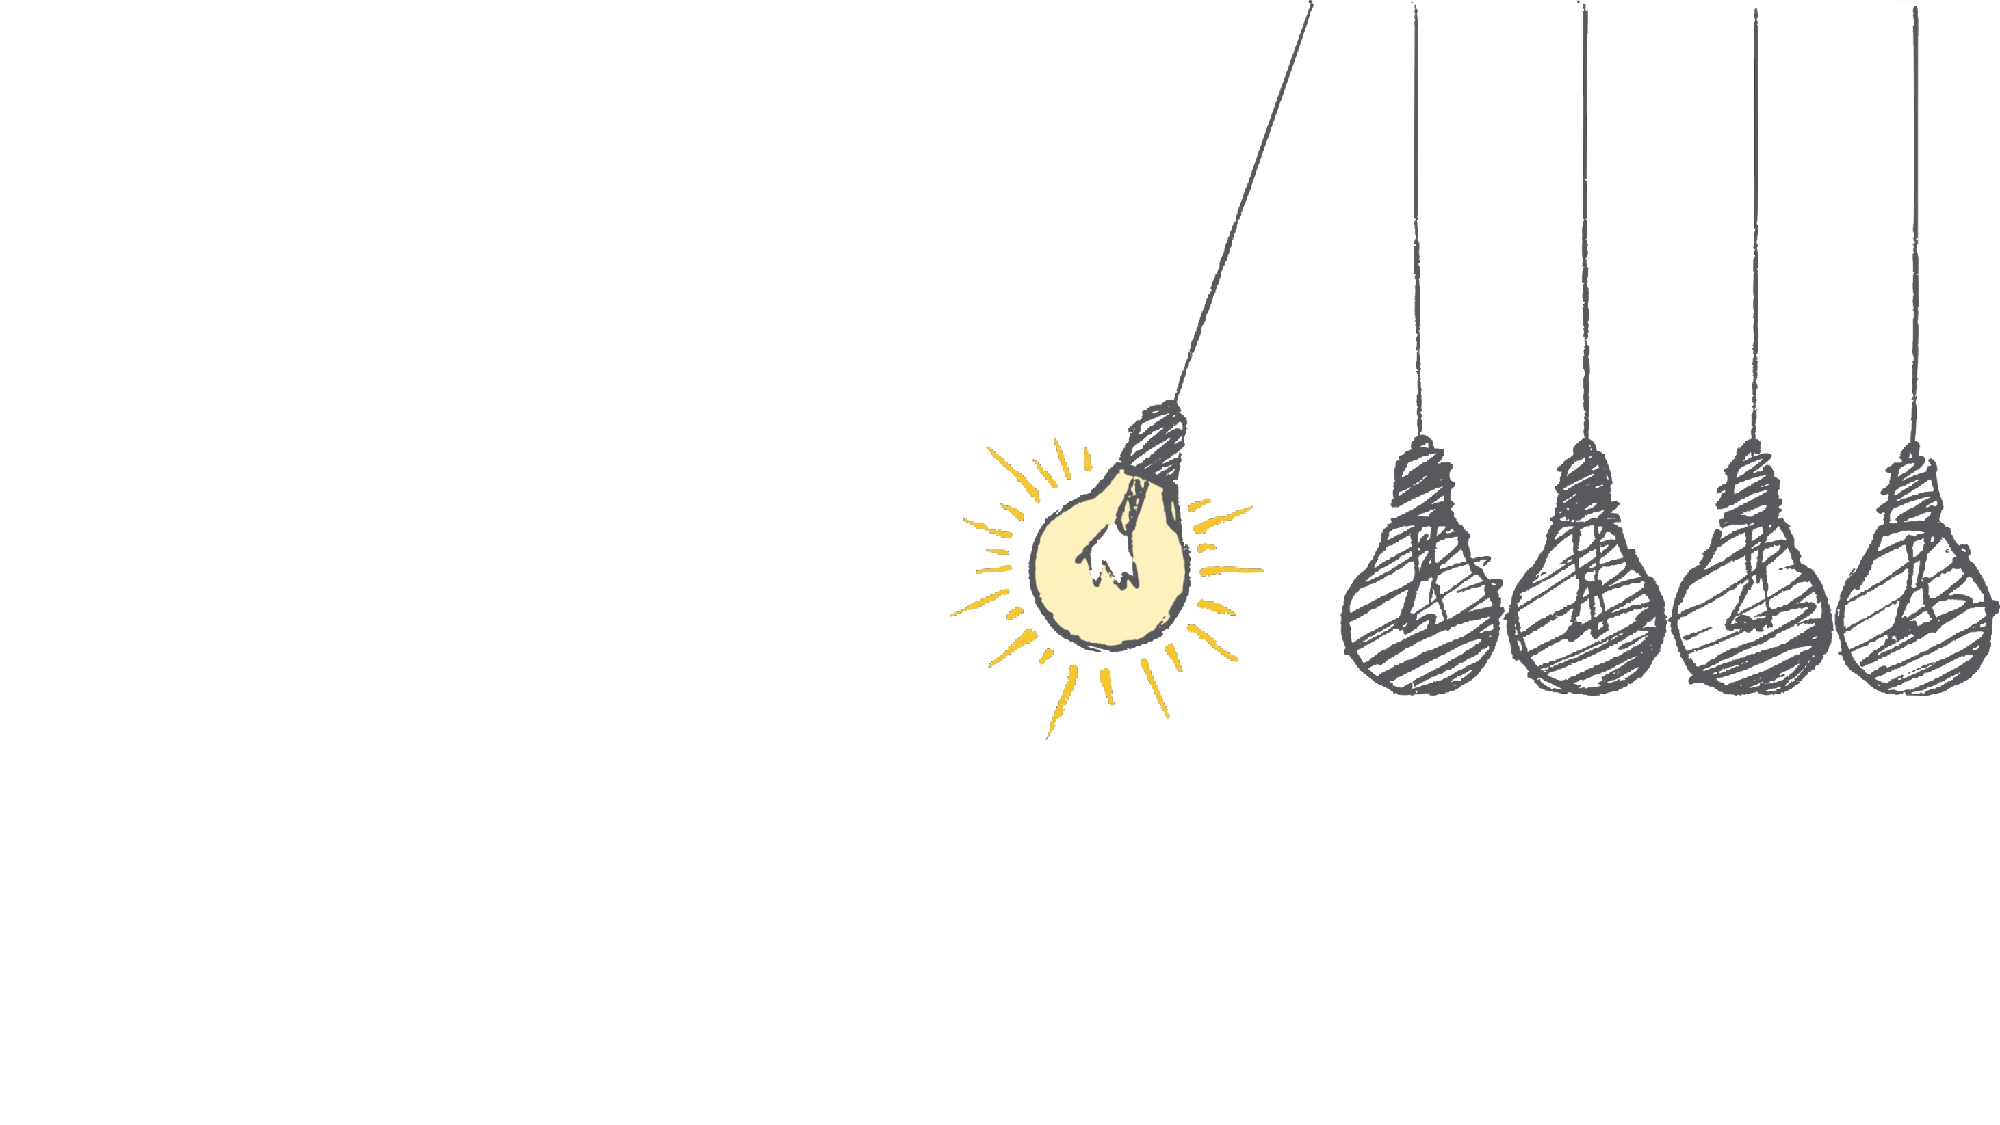
\includegraphics[height=55mm,right]{img/top_right_corner.pdf}} 
		\maketitle
	}

\begin{frame}

	\frametitle{Overview} % Table of contents slide, comment this block out to remove it
	\tableofcontents % Throughout your presentation, if you choose to use \section{} and \subsection{} commands, these will automatically be printed on this slide as an overview of your presentation

\end{frame}

%%%%%%%%%%%%%%%%%%%%%%%%%%%%%%%%%%%%%%%%%%% Section title slide
\sectionpic{Introduction}{img/section_slide}

%%%%%%%%%%%%%%%%%%%%%%%%%%%%%%%%%%%%%%%%%%% Regular slides
\begin{frame}{Introduction}

	\begin{itemize}
		\item This session will introduce you to the basics of Python
		\item In the end we will apply this to a web scraping exercise 
		\item After this session, you'll be able to write and review \textbf{basic} Python code
		\item This session does not include how to use datasets in Python 
		- instead it will focus on the fundamental building blocks to everything in Python,
		data types
	\end{itemize}

\end{frame}

\begin{frame}{Python for Stata users}
	
	\begin{itemize}
		\item There are many great Python courses available for free on the internet - so why is DIME Analytics making yet another one?
		\item This session makes two assumptions not common among the courses already available:
		\begin{itemize}
			\item We assume that you will use Python for research and not computer science
			\item We assume that you are coming from a Stata background 
		\end{itemize}
		\item Many concepts will be explained by referencing concepts in Stata
	\end{itemize}
	
\end{frame}

\begin{frame}{Introduction - Why Python if I already use Stata?}

	\begin{itemize}
		\item Versatility: you can solve almost any programming task with Python:
		\begin{itemize}
			\item Web scraping, text analysis, web applications to retrieve data, machine learning
		\end{itemize}
		\item Much bigger user base
		\item Python is open source and free to use!
		\item Since it's open source it is easier to run everywhere -- for example on big data servers
	\end{itemize}

	However, a big part of the user base does not do research or data science, 
	and libraries for some less frequently used statistical operation 
	has not yet been developed

\end{frame}

%%%%%%%%%%%%%%%%%%%%%%%%%%%%%%%%%%%%%%%%%%% Section title slide
\sectionpic{Getting started}{img/section_slide}

%%%%%%%%%%%%%%%%%%%%%%%%%%%%%%%%%%%%%%%%%%% Regular slides
\begin{frame}{Getting started}

	\begin{itemize}
		\item We'll use Google Colab for this session: https://colab.research.google.com
		\item Colab is similar to a Google doc for coding, and it runs Python by default
	\end{itemize}

\end{frame}

\begin{frame}{Getting started}

	\begin{itemize}
		\item Go to https://colab.research.google.com
		\item Click on \texttt{NEW NOTEBOOK} if you're already logged in, or go to \texttt{File > New notebook} if you're not
	\end{itemize}

	\begin{multicols}{2}

		\begin{figure}
			\centering
			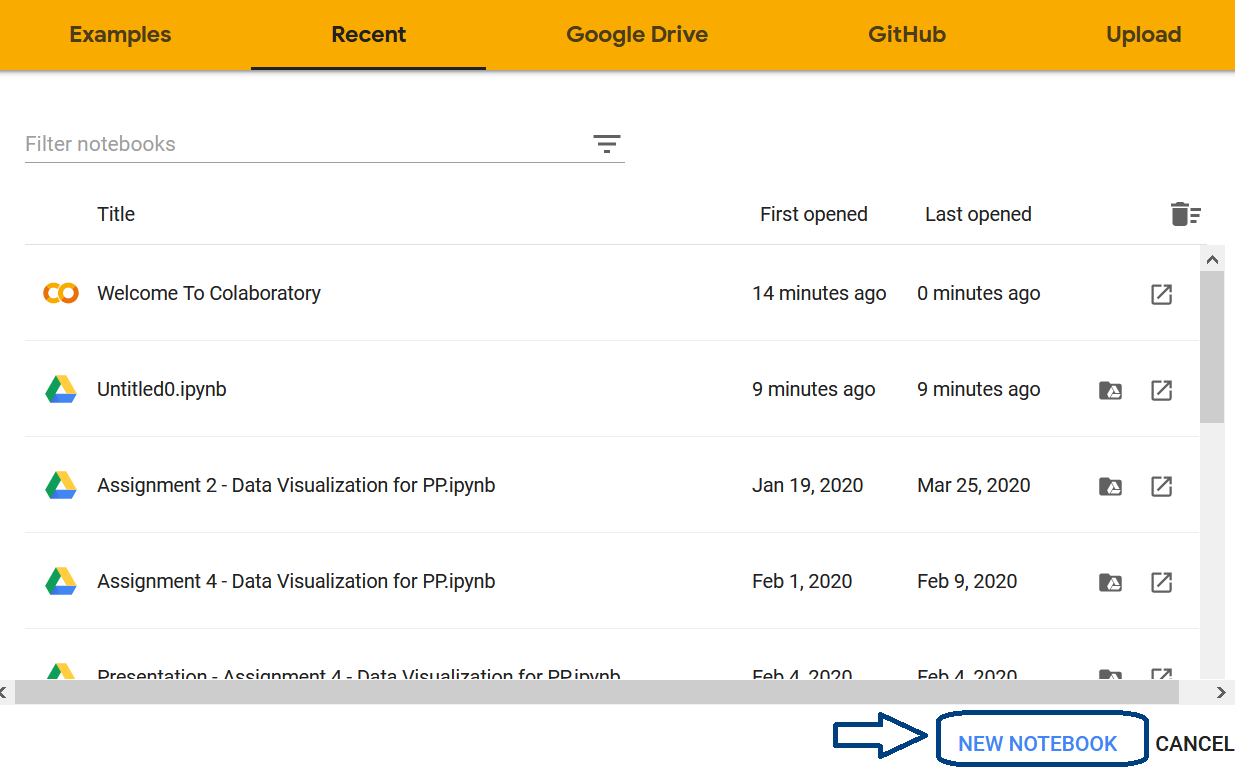
\includegraphics[width=0.9\linewidth]{img/new_nb_logged_in.png}
			\caption{Do this if you're already logged in}
		\end{figure}
		\begin{figure}
			\centering
			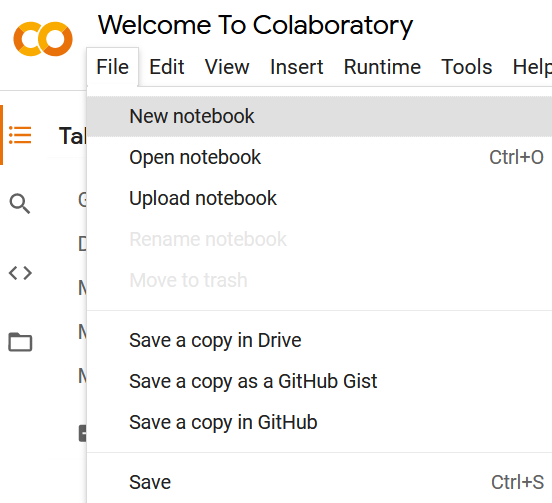
\includegraphics[width=0.6\linewidth]{img/new_nb_not_logged_in.png}
			\caption{Do this if you're not -- you'll be prompted to log in}
		\end{figure}

	\end{multicols}

\end{frame}

\begin{frame}{Getting started - Colab}

	\begin{itemize}
		\item Colab organize code in blocks - each block is like its own script
		\item To run the code in a block, 
		click the $\blacktriangleright$ symbol or press \texttt{Ctrl} + \texttt{Enter}
	\end{itemize}

	\begin{figure}
		\centering
		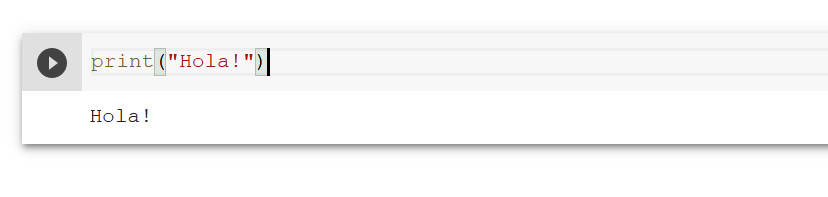
\includegraphics[width=0.6\linewidth]{img/block_of_code.png}
	\end{figure}

	\begin{itemize}
		\item Click on \texttt{+ Code} to add new blocks of code
	\end{itemize}

	\begin{figure}
		\centering
		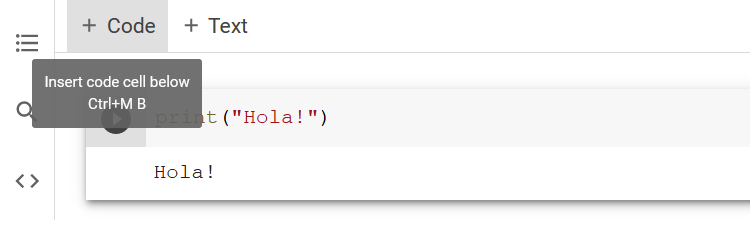
\includegraphics[width=0.6\linewidth]{img/add_code.png}
	\end{figure}

\end{frame}

\begin{frame}{Getting started - Colab}

	\begin{itemize}
		\item You can also add blocks of plain text in Colab by clicking on \texttt{+ Text}
		\item Text blocks are great to explain what you're doing in a code block
	\end{itemize}

	\begin{figure}
		\centering
		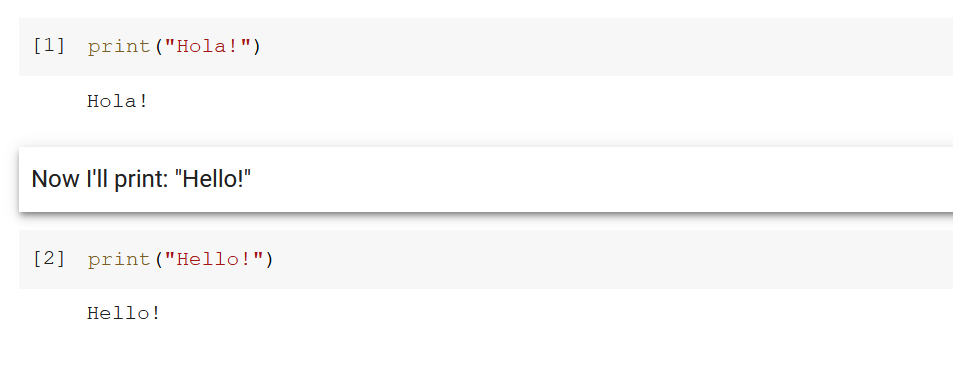
\includegraphics[width=0.6\linewidth]{img/text_block_between_code_blocks.png}
	\end{figure}

	\textbf{Important:} Code and text blocks are a feature specific to Colab. Most Python distributions don't have this feature

\end{frame}

%%%%%%%%%%%%%%%%%%%%%%%%%%%%%%%%%%%%%%%%%%% Section title slide
\sectionpic{Python basic data types}{img/section_slide}

%%%%%%%%%%%%%%%%%%%%%%%%%%%%%%%%%%%%%%%%%%% Regular slides
\begin{frame}{Python basic data types}

	\begin{itemize}
		\item Macros (globals and locals) are often used in Stata to store text or numbers 
		- in Python we use data types, also called objects
		\item However, while macros in Stata are "nice to have", 
		objects in Python are the building block of everything 
		and you cannot write Python code without them
		\item Today we will cover the most basic data types: 
		int/float (numbers), strings, booleans and lists
		\item Data types or objects does more then just store data, 
		the provide operations related to that data type, 
		for example, add and remove item from a list, make a string upper case etc.
		
	\end{itemize}
\end{frame}

\begin{frame}{Python - more on data types}

	\begin{itemize}
		\item Two other common built-in data types not covered today are tuples and dictionaries 
		- but there are an infinite number of other data types or objects
		\item Python users build their own data types based on the built-in types 
		- you will frequently use such data types
		\item For example, data sets in Python is an object called Pandas 
		which is a custom data type implemented by the Python community
		\item All of these custom data types store data 
		and provide operations specially implemented for the intended context
	\end{itemize}
\end{frame}


\begin{frame}{Python basic classes - Defining an object}

	Just like in Stata, the \texttt{=} operator is used to assign value in Python
	
	When we assign value to a data type in Python we say that we create \textit{an object},
	or \textit{an instance of an object}

	\begin{figure}
		\centering
		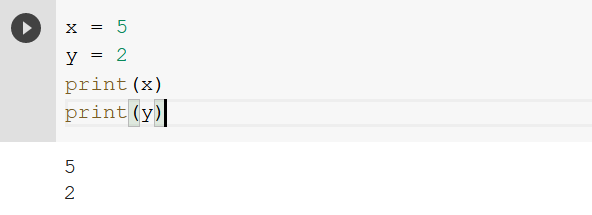
\includegraphics[width=0.6\linewidth]{img/assignation.png}
	\end{figure}

	Note: An instance of an object can also be called \textit{a variable},
	which can be confusing as that term is reserved for a column in a data set in Stata

\end{frame}

\begin{frame}{Python basic classes - \texttt{int}}

	The \texttt{x} and \texttt{y} objects we just defined have the class \texttt{int}

	\begin{figure}
		\centering
		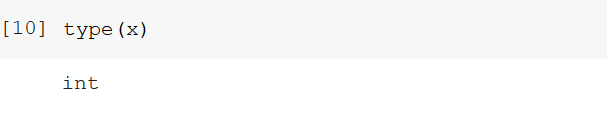
\includegraphics[width=0.6\linewidth]{img/type_int.png}
	\end{figure}

	\texttt{int} objects are integer numbers. We can do mathematical operations with them
	\begin{figure}
		\centering
		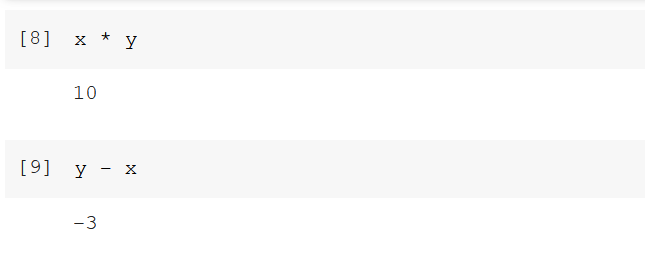
\includegraphics[width=0.6\linewidth]{img/math_integers.png}
	\end{figure}

\end{frame}

\begin{frame}{Python basic classes - \texttt{float}}

	\texttt{float} objects, on the other hand, represent real numbers 
	- we can do mathematical operations with floats as well

	\begin{figure}
		\centering
		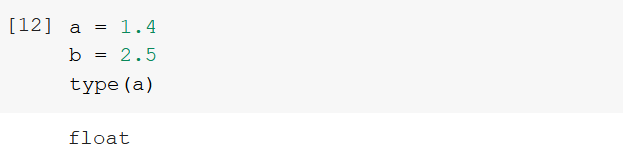
\includegraphics[width=0.6\linewidth]{img/type_float.png}
	\end{figure}

	Python is what's called "\textit{dynamically typed}", 
	which means that you do not need to indicate what data type you want 
	- Python detects if it is an integer, floating point (decimal number), 
	text etc. as long as it is a built-in data type.

\end{frame}

\begin{frame}{Python basic classes - \texttt{str}}

	\texttt{str} objects are strings with text

	\begin{figure}
		\centering
		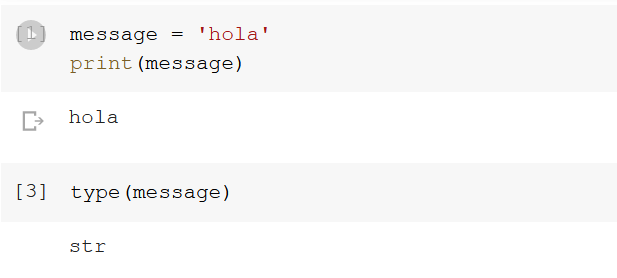
\includegraphics[width=0.6\linewidth]{img/string_type.png}
	\end{figure}

	An object can be used across code blocks 
	- this is common in all notebook styled python interfaces, like Colab

\end{frame}

\begin{frame}{Python basic classes - \texttt{str}}

	Python allows two types of mathematical operations with \texttt{str}: \texttt{+} and \texttt{*}

	\begin{figure}
		\centering
		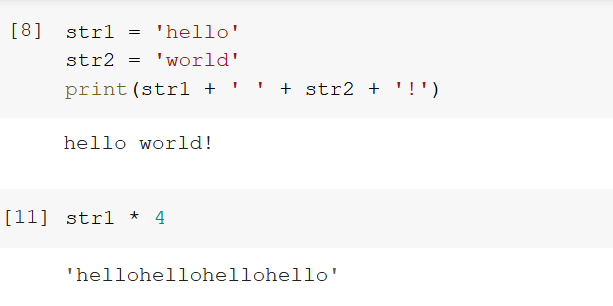
\includegraphics[width=0.6\linewidth]{img/string_operations.png}
	\end{figure}

\end{frame}

\begin{frame}{Python basic classes - \texttt{str}}

	We can also index and create substrings out of \texttt{str} objects

	\begin{figure}
		\centering
		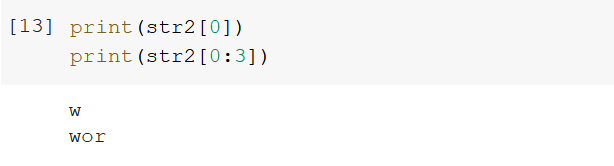
\includegraphics[width=0.6\linewidth]{img/string_indexing.png}
	\end{figure}

	\textbf{Important:}

	\begin{itemize}
		\item Python \textbf{starts indexing at zero}, not at one
		\item When creating a substring with \texttt{a:b}, Python will start by taking the element at position \texttt{a} and will stop at the element \texttt{(b - 1)} -- this is why \texttt{str2[0:3]} returns the letters at positions 0, 1, 2
	\end{itemize}

\end{frame}


\begin{frame}{Python basic classes - Booleans}

	Booleans (\texttt{bool}) are classes representing boolean values -- either \texttt{True} or \texttt{False}

	\begin{figure}
		\centering
		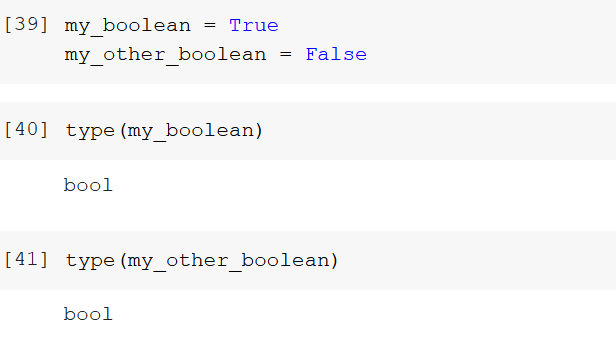
\includegraphics[width=0.6\linewidth]{img/bool.png}
	\end{figure}

\end{frame}

\begin{frame}{Python basic classes - Booleans}

	\begin{itemize}	
		\item We can generate booleans by direct assignation or with boolean expressions
		\item When using direct assignation, Python recognizes booleans when they are written without quotes and with the first character in uppercase and the rest in lowercase
	\end{itemize}

	\begin{figure}
		\centering
		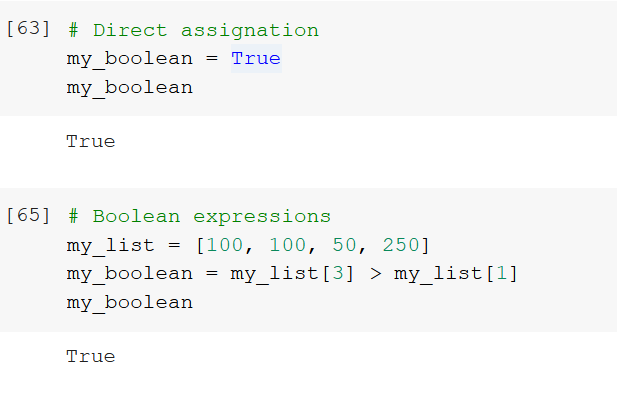
\includegraphics[width=0.6\linewidth]{img/bool_assignation.png}
	\end{figure}

\end{frame}

\begin{frame}{Python basic classes - Booleans}

	Some operators for boolean expressions are \texttt{==}, \texttt{>}, \texttt{>=}, \texttt{<}, \texttt{<=}, and \texttt{in} (to check if an element is part of a list)

	\begin{figure}
		\centering
		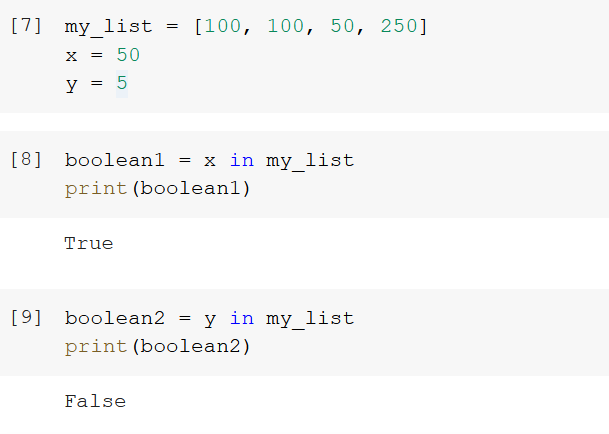
\includegraphics[width=0.6\linewidth]{img/bool_in.png}
	\end{figure}

\end{frame}

\begin{frame}{Python basic classes - Booleans}

	We can do logical operations with booleans using \texttt{and}, \texttt{\&}, \texttt{or}, \texttt{|}

	\begin{multicols}{2}

		\begin{figure}
			\centering
			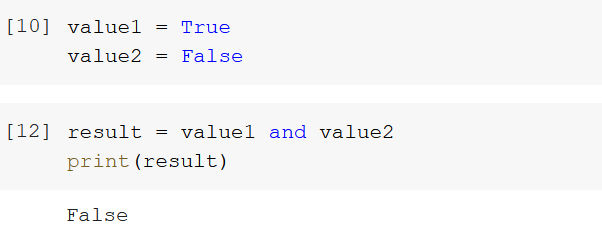
\includegraphics[width=0.8\linewidth]{img/and.png}
		\end{figure}
		\begin{figure}
			\centering
			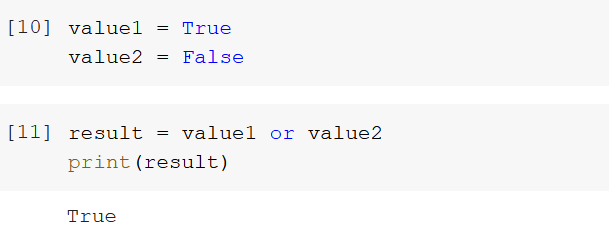
\includegraphics[width=0.8\linewidth]{img/or.png}
		\end{figure}

	\end{multicols}


\end{frame}

\begin{frame}{Python basic classes - Booleans}

	The order of the operations and the use of parenthesis matter for the results. Python will solve first the operations at the beginning of a line and continue one by one until the end unless something is enclosed in parentheses

	\begin{figure}
		\centering
		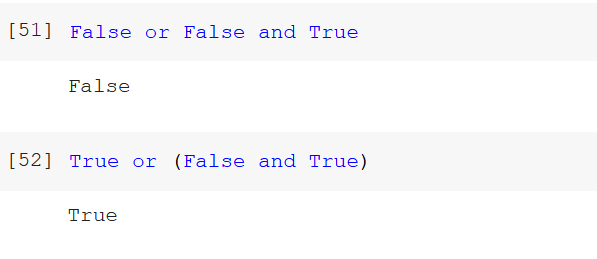
\includegraphics[width=0.6\linewidth]{img/bool_operations.png}
	\end{figure}

\end{frame}

\begin{frame}{Python basic classes - Lists}

	\begin{itemize}
		\item Python uses lists to group objects like \texttt{str}, \texttt{int}, \texttt{float}, and \texttt{bool} into another object
		\item Lists are defined enclosed in brackets and separating its values with commas
	\end{itemize}

	\begin{figure}
		\centering
		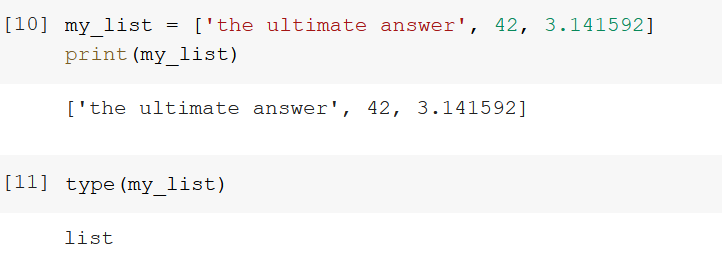
\includegraphics[width=0.6\linewidth]{img/list_type.png}
	\end{figure}

\end{frame}

\begin{frame}{Python basic classes - Lists}

	We can index and subset lists as we did with strings

	\begin{figure}
		\centering
		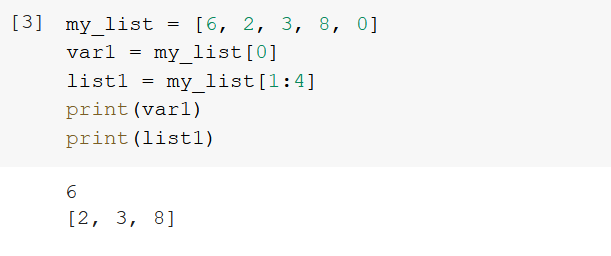
\includegraphics[width=0.6\linewidth]{img/list_subset.png}
	\end{figure}

\end{frame}

\begin{frame}{Python basic classes - Lists}

	To add new elements to existing lists, we use \texttt{.append()}

	\begin{figure}
		\centering
		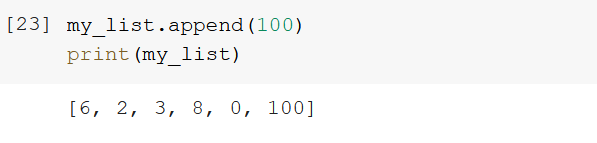
\includegraphics[width=0.6\linewidth]{img/list_append.png}
	\end{figure}

	Note that this will modify our list in-place -- it's not necessary to define the result as a new object when we use \texttt{.append()}

\end{frame}

\begin{frame}{Python basic classes - Lists}

	Python allows for the use of the \texttt{+} and \texttt{*} operators between lists

	\begin{figure}
		\centering
		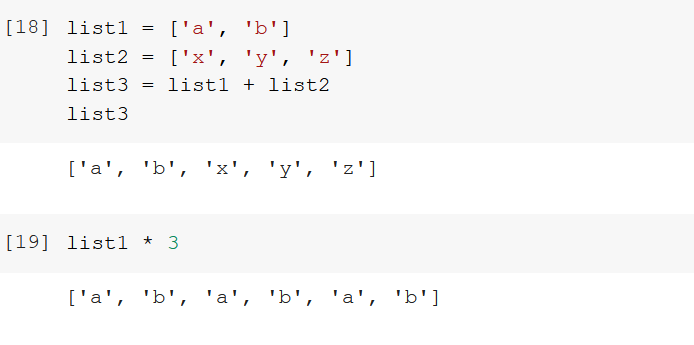
\includegraphics[width=0.6\linewidth]{img/list_operations.png}
	\end{figure}

\end{frame}

\begin{frame}{Python basic classes - Lists}

	Differently to Stata's variables, Python allows to have objects of different classes inside lists. We can even have lists as list elements and use chained indexing.

	\begin{figure}
		\centering
		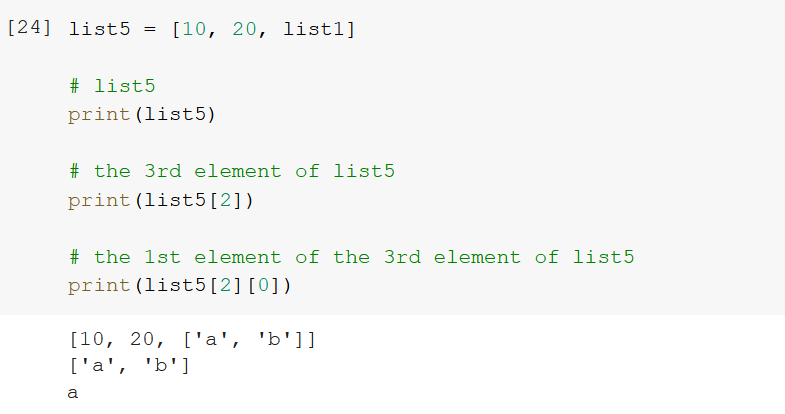
\includegraphics[width=0.6\linewidth]{img/list_many_types.png}
	\end{figure}

\end{frame}

%%%%%%%%%%%%%%%%%%%%%%%%%%%%%%%%%%%%%%%%%%% Section title slide
\sectionpic{Python basic syntax}{img/section_slide}

%%%%%%%%%%%%%%%%%%%%%%%%%%%%%%%%%%%%%%%%%%% Regular slides

\begin{frame}{Basic syntax - Attributes}

	\begin{itemize}
		\item Attributes are:
			\begin{enumerate}
				\item Operations that transform an object in-place
				\item Operations that return a transformation of an object without modifying the original object
			\end{enumerate}
		\item The syntax of attributes is \textit{almost} always: \texttt{OBJECT\_NAME.ATTRIBUTE\_NAME(INPUTS\_IF\_ANY)}
	\end{itemize}

\end{frame}

\begin{frame}{Basic syntax - Attributes}

	\begin{itemize}
		\item \texttt{.append()} is an example of an attribute that transforms an object in-place. It's an attribute of \texttt{list} objects
		\item \texttt{.lower()} is an example of an attribute that returns a modified object without modifying the original object. It's an attribute of \texttt{str} objects
	\end{itemize}

	\begin{figure}
		\centering
		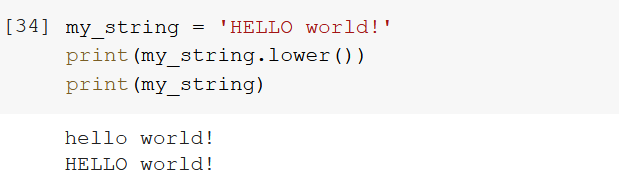
\includegraphics[width=0.6\linewidth]{img/string_lower.png}
	\end{figure}

	\begin{itemize}
		\item Attributes are specific to classes
	\end{itemize}

\end{frame}

\begin{frame}{Basic syntax - Looping}

	We use \texttt{for} and \texttt{in} to loop through an element -- for example, through a list 

	\begin{figure}
		\centering
		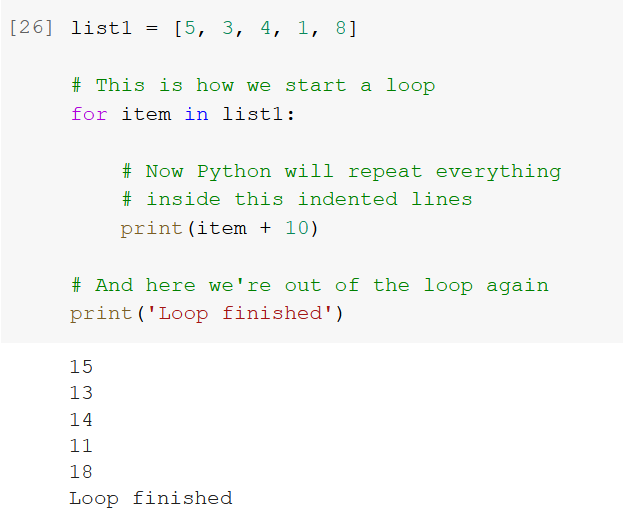
\includegraphics[width=0.6\linewidth]{img/list_loop.png}
	\end{figure}

\end{frame}

\begin{frame}{Basic syntax - Looping}

	\textbf{Important:}

	\begin{itemize}	
		\item Python differentiates what is inside the \texttt{for} loop and where it ends with an indentation space
		\item Indentation can be two spaces or four spaces depending on your text editor or Python tool. In any case, you can also press the \texttt{tab} key to create indented space
		\item If you ever run the script of a colleague who uses different indentation spacing Python will automatically know which indentation to assume. You just have to make sure that indentation is consistent within the same script.
	\end{itemize}

\end{frame}

\begin{frame}{Basic syntax - Looping}

	Lists are not the only class we can loop through. Iterable objects actually include many classes: for example \texttt{str} objects allow us to loop through individual characters

	\begin{figure}
		\centering
		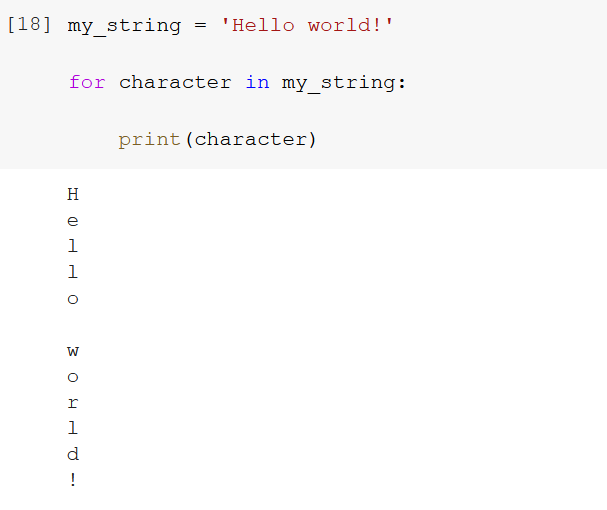
\includegraphics[width=0.55\linewidth]{img/string_loop.png}
	\end{figure}

\end{frame}

\begin{frame}{Basic syntax - \texttt{if}, \texttt{elif}, \texttt{else}}

	\texttt{if}, \texttt{elif}, and \texttt{else} are used to define conditional operations

	\begin{multicols}{3}

		\begin{figure}
			\centering
			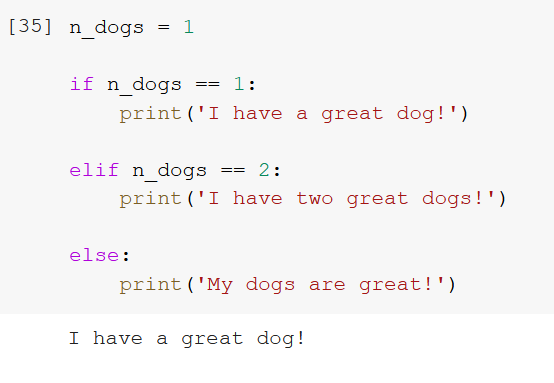
\includegraphics[width=\linewidth]{img/if.png}
		\end{figure}
		\begin{figure}
			\centering
			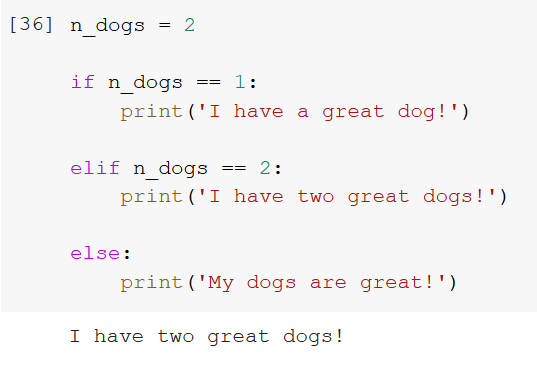
\includegraphics[width=\linewidth]{img/elif.png}
		\end{figure}
		\begin{figure}
			\centering
			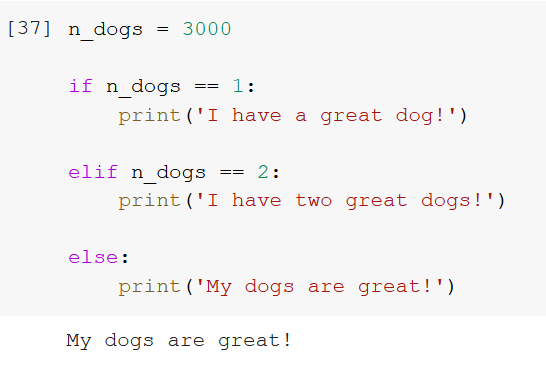
\includegraphics[width=\linewidth]{img/else.png}
		\end{figure}

	\end{multicols}

\end{frame}

\begin{frame}{Basic syntax - \texttt{if}, \texttt{elif}, \texttt{else}}

	\begin{itemize}
		\item A boolean expression or a boolean value must be used with \texttt{if} and with \texttt{elif}
		\item \texttt{if} doesn't necessarily need to be used with \texttt{elif} of with \texttt{else}, but these two should always be preceded by \texttt{if}
	\end{itemize}

	\begin{multicols}{3}

		\begin{figure}
			\centering
			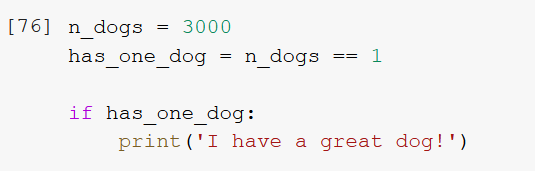
\includegraphics[width=\linewidth]{img/if_alone.png}
		\end{figure}
		\begin{figure}
			\centering
			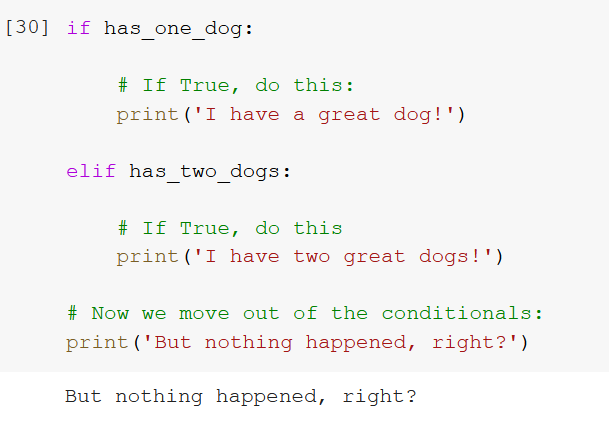
\includegraphics[width=\linewidth]{img/if_elif.png}
		\end{figure}
		\begin{figure}
			\centering
			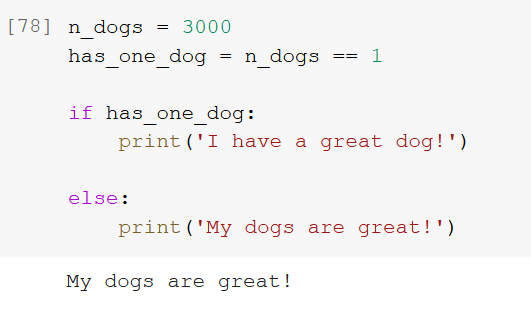
\includegraphics[width=\linewidth]{img/if_else.png}
		\end{figure}

	\end{multicols}

	\begin{itemize}
		\item Note that the first two examples will not apply any operation because none of the values of the objects after \texttt{if} or \texttt{elif} is \texttt{True}.
		\item Both \texttt{if}, \texttt{elif}, and \texttt{else} need to have the same indentation level
	\end{itemize}

\end{frame}

\begin{frame}{Basic syntax - \texttt{if}, \texttt{elif}, \texttt{else}}

	\begin{itemize}
		\item If a boolean expression returned \texttt{True} for conditions in both \texttt{if} and \texttt{elif}, only the operations  under \texttt{if} would be executed
		\item If more than one boolean expression under several \texttt{elif} conditions were to return \texttt{True}, only the operations under the first \texttt{elif} condition evaluated to \texttt{True} would be executed
	\end{itemize}

	\begin{multicols}{2}

		\begin{figure}
			\centering
			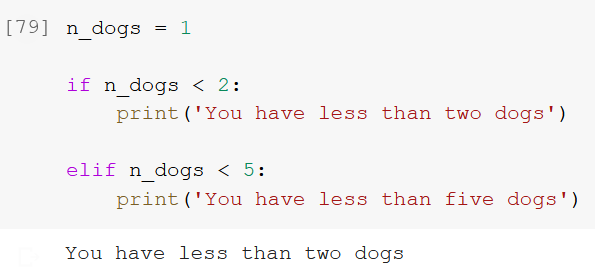
\includegraphics[width=\linewidth]{img/if_and_elif_true.png}
		\end{figure}
		\begin{figure}
			\centering
			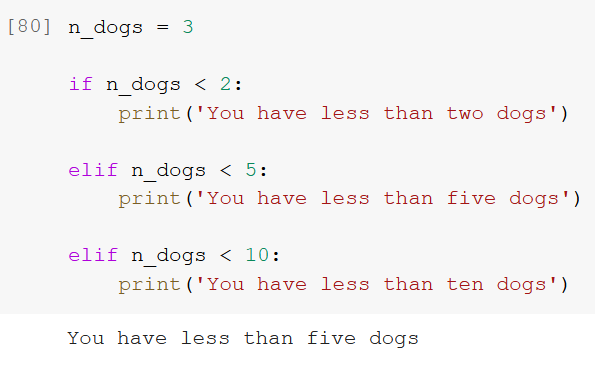
\includegraphics[width=\linewidth]{img/elif_and_elif_true.png}
		\end{figure}

	\end{multicols}

\end{frame}

\end{document}